%%%%%%%%%%%%%%%%%%%%%%%%%%%%%%%%%%%%%%%%%%%%%%%%%%%%%%%%%%%%%%%%%
% Contents: The QIF chapter
% $Id: grisbi-manuel-QIF.tex, v 0.4 2002/10/27 Daniel Cartron
% $Id: grisbi-manuel-QIF.tex, v 0.5.0 2004/06/01 Loic Breilloux
% $Id: grisbi-manuel-QIF.tex, v 0.6.0 2011/11/17 Jean-Luc Duflot
% $Id: grisbi-manuel-QIF.tex, v 0.8.9 2012/04/27 Jean-Luc Duflot
% $Id: grisbi-manuel-QIF.tex, v 1.0 2014/02/12 Jean-Luc Duflot
%%%%%%%%%%%%%%%%%%%%%%%%%%%%%%%%%%%%%%%%%%%%%%%%%%%%%%%%%%%%%%%%%


\chapter{Export and import of accounts\label{move}}

You can not directly use data that has been created by other personal accounting applications in Grisbi, and vice versa. Because these applications work differently, their data is structured differently, so you need to convert their data structure before you can use it. 

This conversion can not be done at once on all data, but must be done separately for each account managed by the application. To convert each of these accounts, you must first \og export \fg{}them from the original application and then \og import \fg{} them into the destination application.

% espace avant Attention ou Note  : 5 mm
\vspacepdf{5mm}

\strong{Warning} :  do not confuse the \og accounts file \fg{}which contains all the data of all the accounts created for the management of an accounting entity (in Grisbi, this file has the \gls{extension} \file{.gsb}), and the \og account files\fg{}, which are files that contain only data from one account at a time, and created only to export or import that data from one accounting application to another. These \og account files  \fg{}  must have a  \gls{file format} (or extension) that must be compatible with the original application AND the destination application.
% espace après Attention ou Note  : 5 mm
\vspacepdf{5mm}

Grisbi currently supports \gls{Gnucash}, \gls{OFX}, \gls{CSV} and \gls{QIF} personal accounting data formats.

\section{Importing accounts from another accounting application\label{move-import}}

If you want to use account data that has been created
in another accounting application in Grisbi, you must first export each of the accounts of this application individually to a set of files, then import these same files into Grisbi.

\subsection{Export an account file from the other accounting application \label{move-import-exportinit}}

The first step is, in the originating personal accounting application, to export each account in a file in the chosen format. The chosen format must be compatible with the export formats supported by the original application \emph{and} compatible with import to Grisbi.

The export procedure is obviously different for each accounting application, so refer to its documentation. If you want to export all accounts, you will need to get as many files as you have accounts managed by the application.


\subsection{Importing account files from another accounting application to Grisbi\label{move-import-importinit}}

\textbf{Note} : Grisbi allows you to import one or more account files in one operation. Although you can import the account files one by one, it is important to import all the account files at the same time, so that Grisbi can recreate the links between the accounts, especially with regard to the transfer operations.
% espace après Attention ou Note  : 5 mm
\vspacepdf{5mm}

For more information on the \indexword{account types}\index{types de compte} that Grisbi can manage, see the \vref{accounts-type}, \menu{Grisbi account types} section.

You can define which date will be used for assigning a financial year to
each imported operation, see \vref{setup-general-import-financialyear}, \menu{Definition of Financial Year}.

When you import a file, Grisbi allows you to establish an association between a string of characters in this file and a payee. For example, all labels containing \og rent \fg{}  may be associated with a payee that represents your landlord. This must be configured in the \menu{Edit - Preferences } menu (see the \vref{setup-general-importLinks}, \menu{Associations for Import} section).

% espace pour changement de thème
\vspacepdf{5mm}

In the Grisbi \menu{File} menu, choose the option  \menu{Import
file\ldots{ }}, which opens the import wizard window. The import of the account files takes place in five steps :

\begin{enumerate}
	\item Launches the import assistant; confirm with the \menu{Forward} button;
	\item Selection of the account files to import :	
		\begin{enumerate}
			\item click the button \menu{Add file to import} button : a file manager window opens,	
			\item look for the directory where these account files are,
			\item select one or more account files (with the combination   \key{Ctrl}\key{Click} and \key{Shift}\key{Click}); you can also change the \gls{locale} (\gls{character encoding}) of the files to import from the \menu{Encoding} drop-down menu,
			\item validate the window to return to the account file selection window,
			\item when the desired files are checked, you can validate the selection with the \menu{Forward} button;
		\end{enumerate}		  
	\item Complete the import of the files: if everything went well, this window gives the list of the account files which will be imported; continue the import by confirming with the \menu{Forward} button;
	\item Review: you can review each account and choose the following actions \strong{Translators Note:} this paragraph has not been checked against Grisbi so could still contain translation errors \ifIllustration \refimage{QIF-import-files-setup-img} :
	% image centrée
	\begin{figure}[htbp]
	\begin{center}
	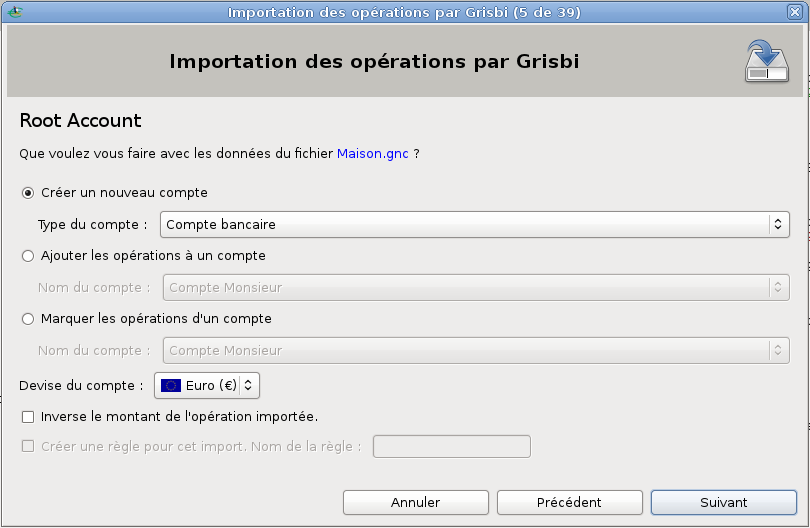
\includegraphics[scale=0.5]{image/screenshot/QIF_import_files_setup}
	\end{center}
	\caption{Setting up each imported account}
	\label{QIF-import-files-setup-img}
	\end{figure}
	% image centrée
	\else  :
	\fi
	
		\begin{itemize}
			\item create a new account,
			\item add a scheduled transaction to an account: If scheduled transactions are found within the specified time interval, a specific window opens to find out what you want to do: either merge these scheduled transaction with the corresponding imported entry, or add them imported transaction in addition to those (see \vref{setup-general-import-parameters}, \menu{Import Settings}),
			\item check the scheduled transactions : if there are \indexword{orphaned transactions}\index{opération !orpheline}  a window will open at the end of the import to know what you want to do: either add them or ignore them,
			\item set the currency of the account (or create a new one),
			\item   reverse the amount of the transaction (useful for credit card accounts for example),
			\item create a fast import rule if the file is in QIF or OFX format,
			\item when everything is correct, confirm the import with the \menu{Next} button;
		\end{itemize}
	
	 \item Confirm the end of the import: confirm with the \menu{Close} button.
\end{enumerate}

If, and only if you have created your account file just before this account data import, return to the end of the  \vref{start-newfile-end}, \menu{Creating a New Account File}. Go directly to the end of the account file creation process, at the paragraph beginning with \emph{In one way or another\ldots{ }}, which will prompt you to create other accounts right away.

%espace pour changement de thème
\vspacepdf{5mm}
Otherwise, you can start using the account you just created.

\section{Export accounts from Grisbi\label{move-export}}

If you want to use account data created by Grisbi in another accounting application, you must first export this data to files and then import them into the other application using these files. The file format chosen must be compatible with the export by Grisbi \emph{and} compatible with the import by the destination application.
 
In the \menu{File} menu select the \menu{Export accounts as QIF/CSV file\ldots{ }} that opens the Export Accounts Wizard. There are four steps to exporting accounts:

\begin{enumerate}
	\item Starting the assistant; this window indicates that, since the QIF and CSV file formats do not support currency, all transactions will be converted into the currency of their respective account; confirm with the \menu{Forward} button;
	\item Select the accounts to export by clicking in the corresponding box; confirm with the  \menu{Forward} button;
	\item For each account, define the name of the file, the destination directory and the export format, then validate with the \menu{Forward} button \ifIllustration \refimage{QIF-export-img} ;
	% image centrée
	\begin{figure}[t]
	\begin{center}
	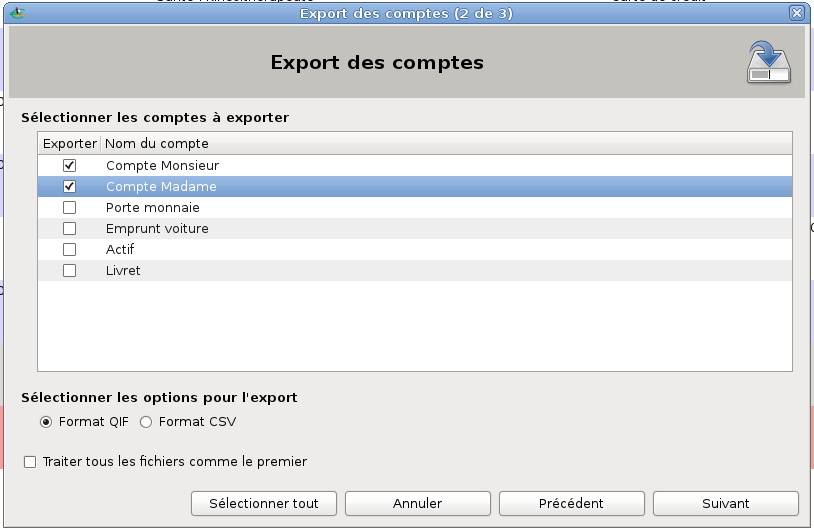
\includegraphics[scale=0.5]{image/screenshot/QIF_export}
	\end{center}
	\caption{Acount export}
	\label{QIF-export-img}
	\end{figure}
	% image centrée
	\else  ;
	\fi
	
	\item The completion of the export window is displayed; confirm with the \menu{Close} button.
\end{enumerate}

\strong{Warning}: in general, it is inadvisable to have accents or spaces in the names of directories and files used by Grisbi. If so, rename them now. For example, spaces can be replaced by underscores (\_).











